\cleardoublepage
\chapter{Results}
\label{ch:results}

This chapter aims at presenting and discussing the results achieved in the ImageCLEF LMRT challenge. Firstly, in Section \ref{sec:first} a few examples of some tests that showcase the fine-tuning of the system are presented. Secondly, in Section \ref{sec:example} an example on how the system performed in a given topic is showcased and some insight is given on the differences in performance between the submitted runs. Finally, in Section \ref{sec:perfomance_results} the results achieved on the challenge are presented.

\section{System Fine-Tuning Using The Dev Topics}
\label{sec:first}

The first tests using the system architecture described on the previous chapter were run on a laptop. The dataset of pictures used was smaller (20.000 images) and not all topics were fully analysed. This tests took between 8h-10h each and they were done in order to find a good weight distribution between each category, detect bugs on the code and overall fine-tune the system before sending the code to the main processing computer (where the fully processing of the dataset took up to 1-2 days).


\begin{figure}[H]
  \centering
  \captionsetup{justification=centering}

  \begin{subfigure}{0.22\textwidth}
  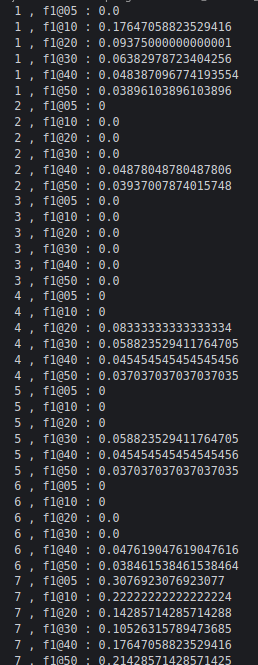
\includegraphics[width=\textwidth]{Sections/7Results/images/runexample5.png} 

  \end{subfigure}
  \begin{subfigure}{0.22\textwidth}
  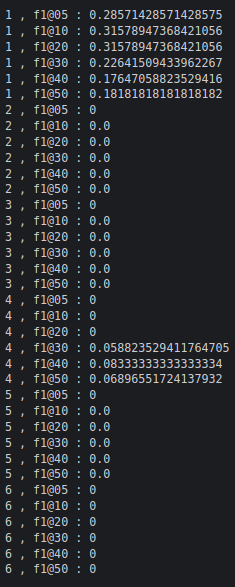
\includegraphics[width=\textwidth]{Sections/7Results/images/runexample3.png}\hfill
  \end{subfigure}
  \begin{subfigure}{0.22\textwidth}
  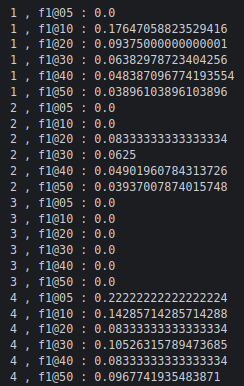
\includegraphics[width=\textwidth]{Sections/7Results/images/runexample4.png}\hfill
  \end{subfigure}
  \caption[Fine-tuning results examples.]{Examples of some different results with the fine-tuning of the weight distribution.}
  \label{fig:fine_tuning}
\end{figure}


The examples in Figure \ref{fig:fine_tuning} show the different achieved performances of the system in the F1-measure@XX during testing. In some cases the importance weight factor attributed to specific categories might be higher or lower, in other cases the general thresholds were changed and in other cases the negative categories were discarded. This tests were conducted during various days with the objective of using the case where the scores were better for the processing of the full dataset. However, since only a small sample of the dataset was processed during testing and fine-tuning, there were no guarantees that having good results during testing would produce good results when processing the full dataset.



\section{Final System Performance Example}
\label{sec:example}

After computing all confidence scores for every image and every topic, the system generates an csv file used for evaluation. The file is organized in the following way: \textbf{[topic id number, image name, confidence score]}. The 50 highest scoring pictures for each topic are stored in this file, however only the 10 highest pictures for each topic are used for the challenge evaluation. An excerpt showing the performance of both runs in test topic 9 is presented in Figure \ref{fig:runs_csv}. This will be further discussed in Section \ref{sec:analysis}.


\begin{figure}[H]
  \centering
  \captionsetup{justification=centering}

  \begin{subfigure}{0.4\textwidth}
  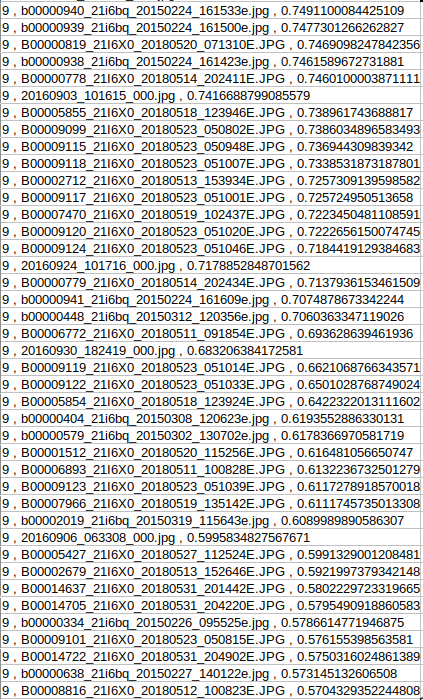
\includegraphics[width=\textwidth]{Sections/7Results/images/topic9_results.png} 
  \caption{Run 1}
  \end{subfigure}
  \hspace{+5mm}
  \begin{subfigure}{0.385\textwidth}
  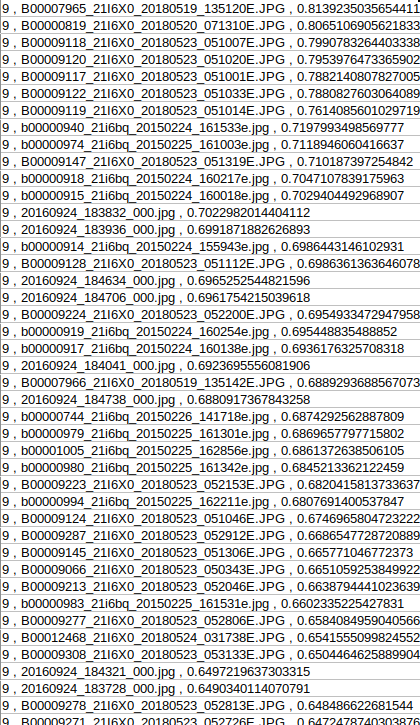
\includegraphics[width=\textwidth]{Sections/7Results/images/topic9results2.png}
  \caption{Run 2}
  \end{subfigure}
  \caption{Achieved results on topic 9 of the test topics.}
  \label{fig:runs_csv}
\end{figure}

\subsection{Topic 9 Performance Analysis}
\label{sec:analysis}

In order to critical analyse the retrieved images from both runs it is important to understand the moment described in topic 9, which is presented next:\\



\textbf{Title}: \enquote{Eating pizza}.

\textbf{Description}: \enquote{Find the moments when u1 was eating a pizza
while talking to one man}.

\textbf{Narrative}: \enquote{To be considered relevant, the u1 must eat or
hold a pizza with a man visible in the background. The moments that
u1 was talking to more than one person are not relevant}.\\


Analysing the images retrieved by both runs for topic 9 (illustrated in Figure \ref{fig:run1} and \ref{fig:run2}) it is clear that run 1 achieved better performance for this specific topic, since 3 of the top 10 images returned belong to the moment described while for run 2 only 2 images from the top 10 belong to the moment. 


As shown in Figure \ref{fig:run1} for run 1 the  top 1, 2 and 4 all belong to the moment since all of these images show the user eating pizza with a man visible in the background. Furthermore, the top 5 image from run 1 also shows the user with a pizza in the background, however there is no man in the background. Subsequently, the top 6 image has a poster of a pizza. Image top 7,8,9 and 10 are not related to the moment at all, however all of the pictures are inside interiors and illustrate food which is similar to the description of the moment.

  
For run 2 (represented in Figure \ref{fig:run2}), the top 8 and 9 are images that are related to the topic, since both of them also show the user eating pizza with a man on the background. All of the other images are related to food being eaten inside an interior, however they do not belong to the described moment. Top 1 and top 2 images show an image of a lasagne which is similar to pizza where the scenario can be considered identical.

Some possible reasons that lead run 1 to achieve better performance than run 2 are presented next:

\begin{itemize}
  \itemsep0em
  \item The negative categories on run 1 might have decreased the confidence score on  pictures that don't belong to the topic.
  \item The object detection algorithm on run 1 might have provided better detections than the algorithm used for run 2.
  \item The category weight distribution on run 2 might have decreased the weight on some categories that were important for the confidence score calculation in the images that belong to the topic.
  \item The difference in the similarity score between the different visual concepts on each run might also impact the performance of the system.
\end{itemize}

\newpage

\begin{figure}[H]
  \centering
  \captionsetup{justification=centering}

  \begin{subfigure}{0.32\textwidth}
    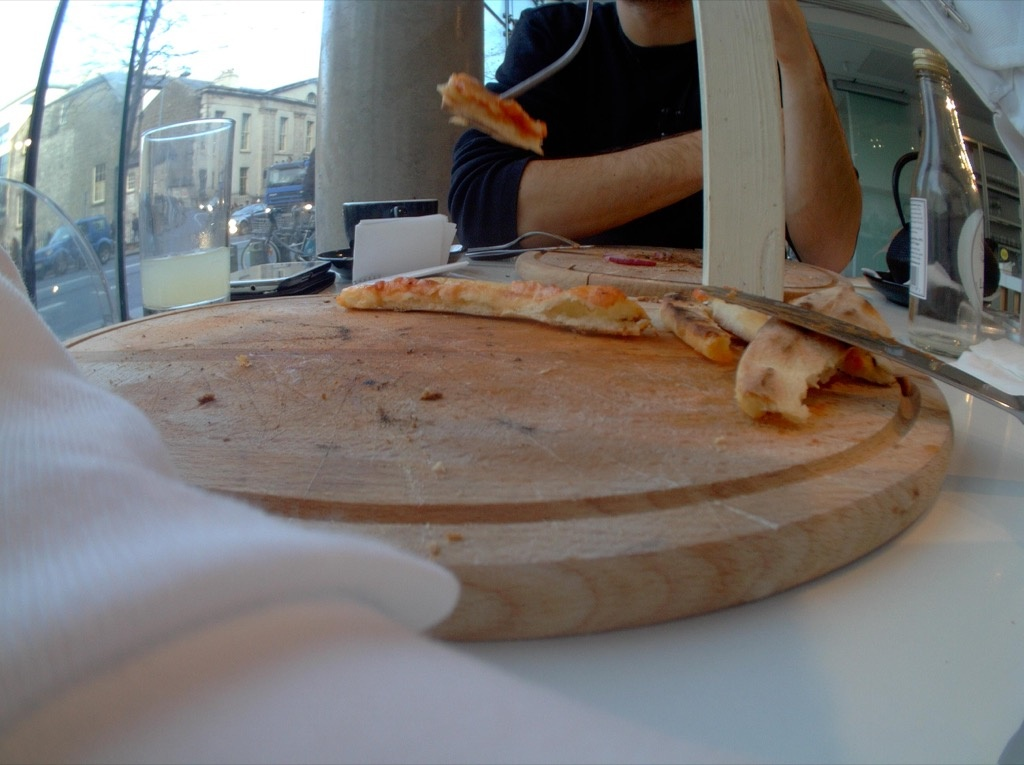
\includegraphics[width=\textwidth]{Sections/7Results/images/top1.jpg} 
    \caption{Top 1}
  \end{subfigure}
  \begin{subfigure}{0.32\textwidth}
    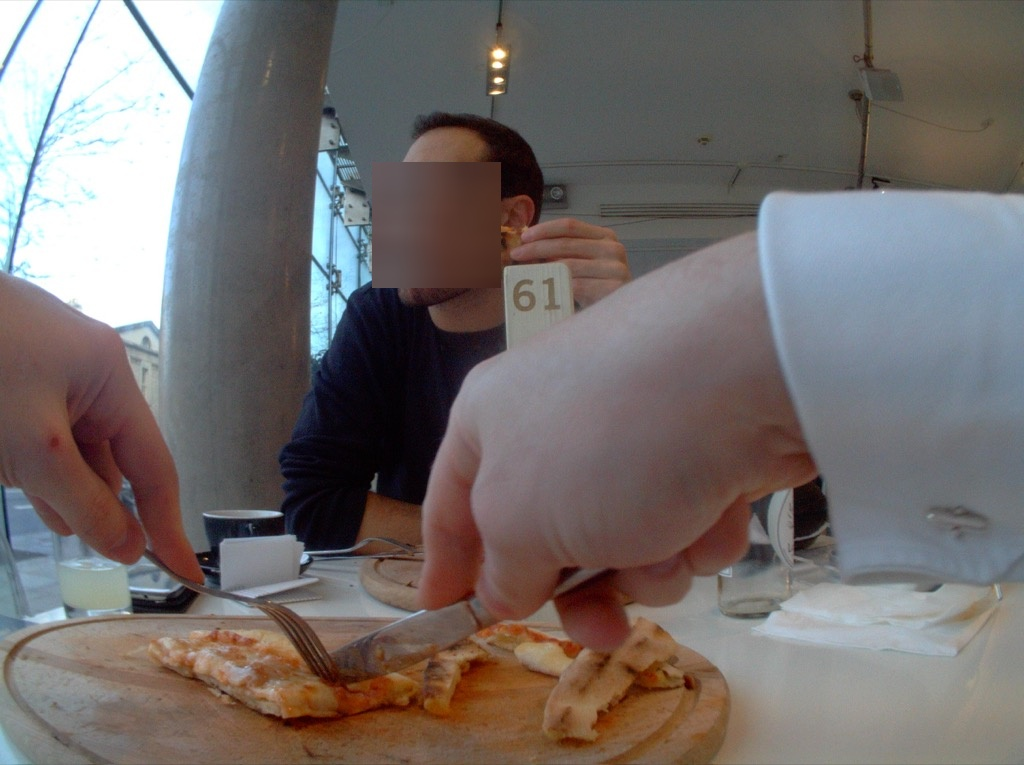
\includegraphics[width=\textwidth]{Sections/7Results/images/top2.jpg}\hfill
    \caption{Top 2}
  \end{subfigure}
  \begin{subfigure}{0.32\textwidth}
    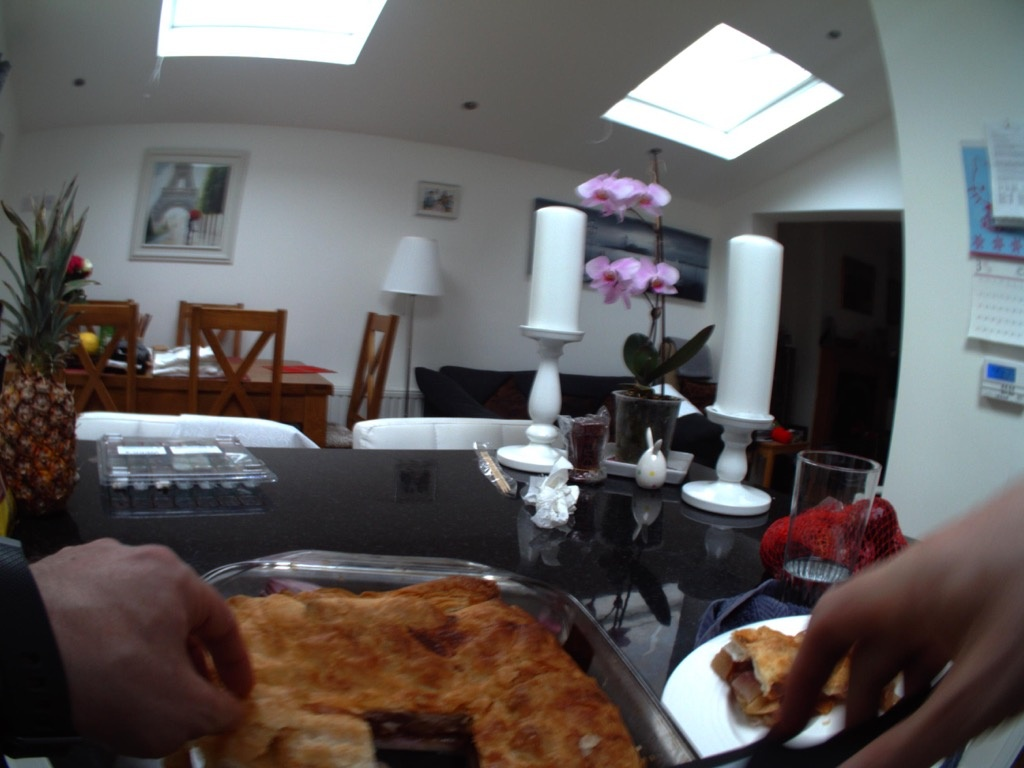
\includegraphics[width=\textwidth]{Sections/7Results/images/top3.jpg}\hfill
    \caption{Top 3}
  \end{subfigure} \par\medskip

  \begin{subfigure}{0.32\textwidth}
    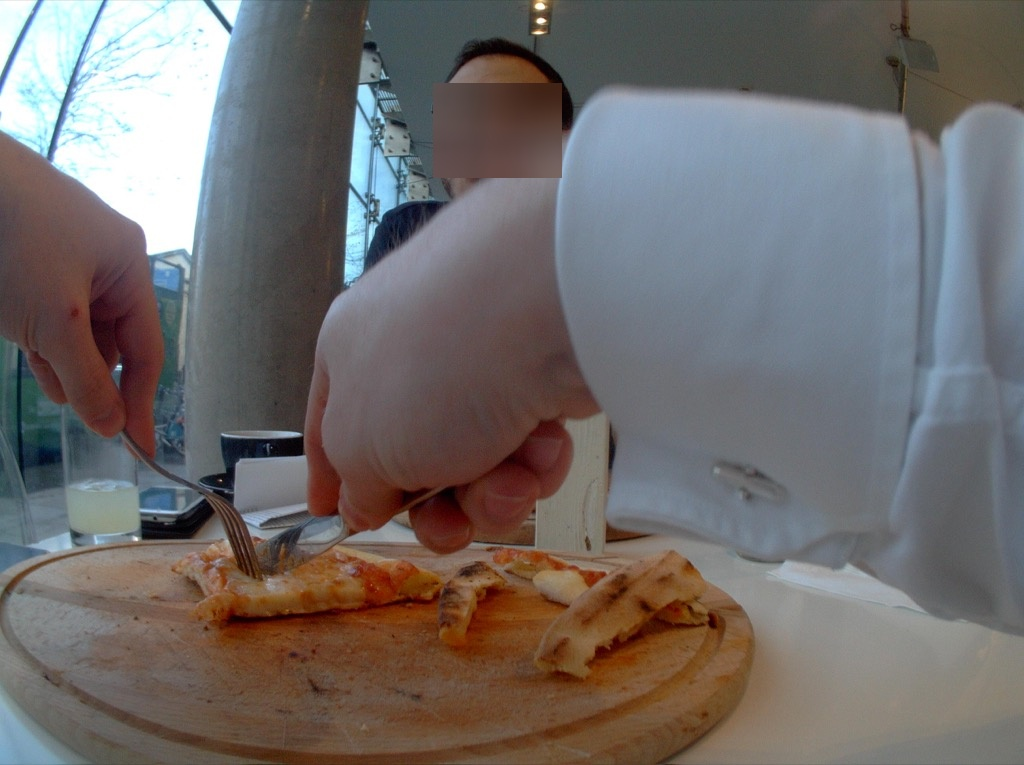
\includegraphics[width=\textwidth]{Sections/7Results/images/top4.jpg}\hfill
    \caption{Top 4}
  \end{subfigure}
  \begin{subfigure}{0.32\textwidth}
    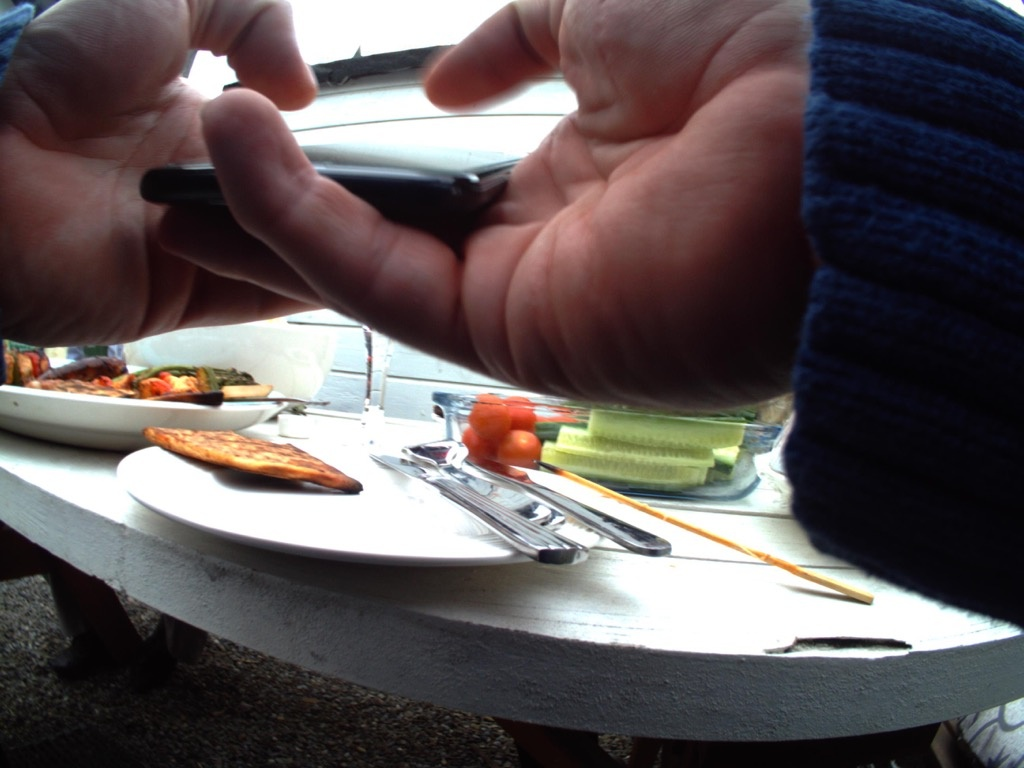
\includegraphics[width=\textwidth]{Sections/7Results/images/top5.jpg}\hfill
    \caption{Top 5}
  \end{subfigure}
  \begin{subfigure}{0.32\textwidth}
    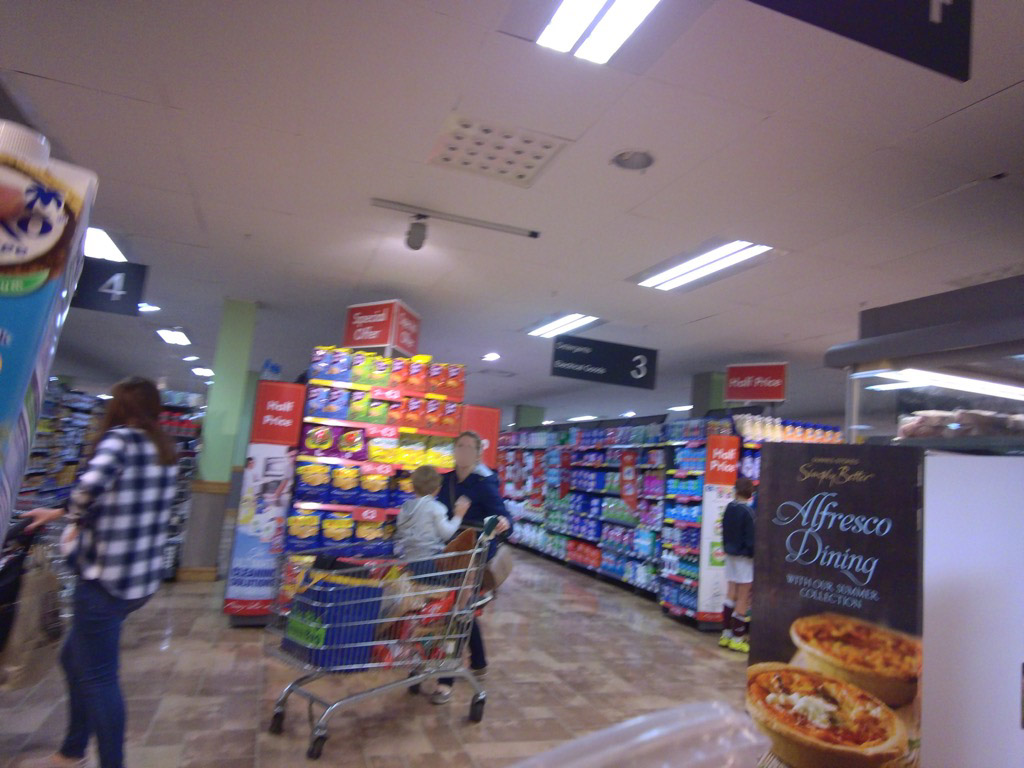
\includegraphics[width=\textwidth]{Sections/7Results/images/top6.jpg}\hfill
    \caption{Top 6}
  \end{subfigure}\par\medskip

  \begin{subfigure}{0.32\textwidth}
    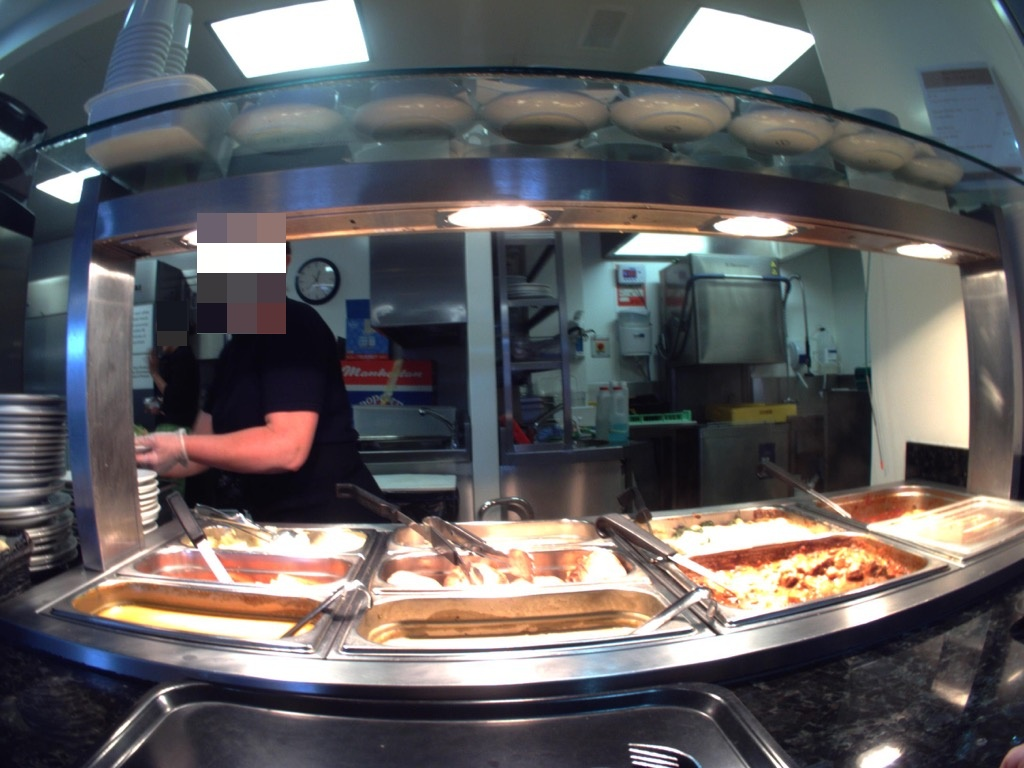
\includegraphics[width=\textwidth]{Sections/7Results/images/top7.jpg} 
    \caption{Top 7}
  \end{subfigure}
  \begin{subfigure}{0.32\textwidth}
    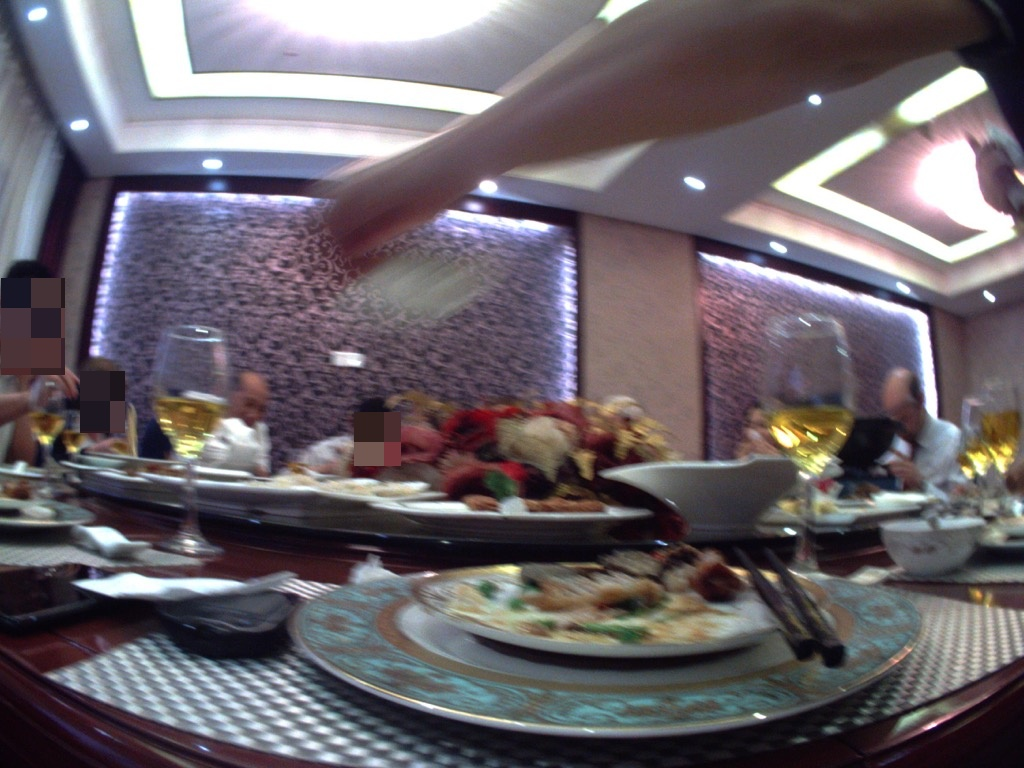
\includegraphics[width=\textwidth]{Sections/7Results/images/top8.jpg}\hfill
    \caption{Top 8}
  \end{subfigure}
  \begin{subfigure}{0.32\textwidth}
    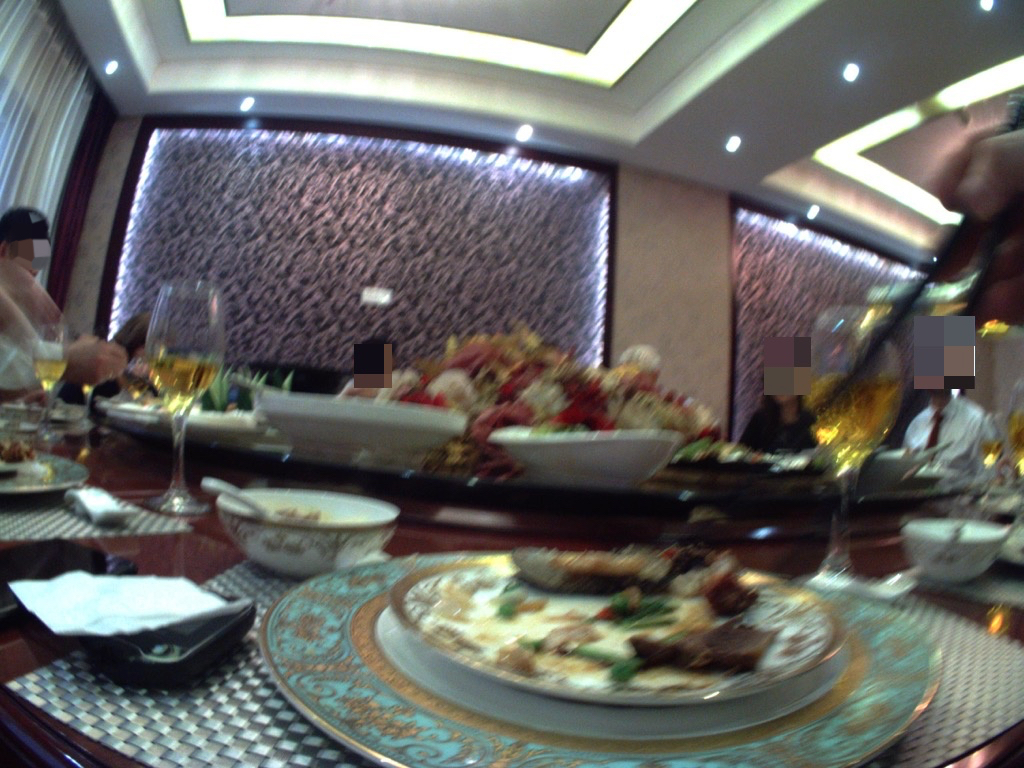
\includegraphics[width=\textwidth]{Sections/7Results/images/top9.jpg}\hfill
    \caption{Top 9}
  \end{subfigure} \par\medskip

  \begin{subfigure}{0.32\textwidth}
    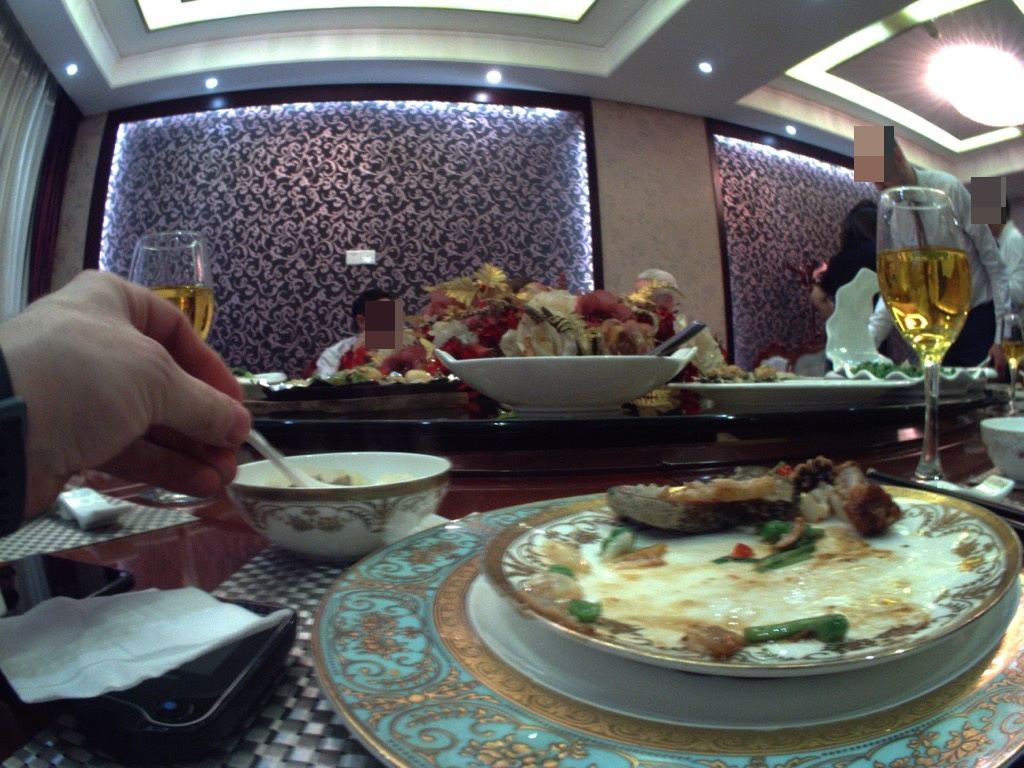
\includegraphics[width=\textwidth]{Sections/7Results/images/top10.jpg}\hfill
    \caption{Top 10}
  \end{subfigure}
  
  \caption{Top 10 retrieved pictures for topic 9 on run 1}
  \label{fig:run1}
\end{figure}




\newpage

\begin{figure}[H]
    \centering
    \captionsetup{justification=centering}
  
        \begin{subfigure}{0.32\textwidth}
          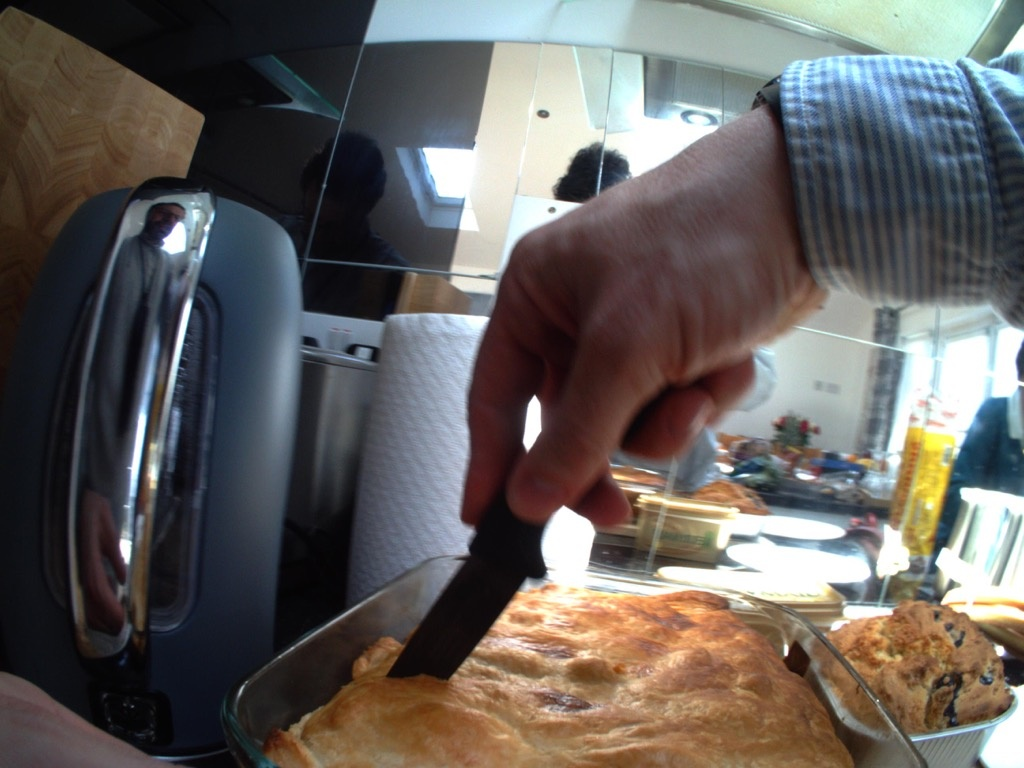
\includegraphics[width=\textwidth]{Sections/7Results/images/run2top1.jpg} 
          \caption{Top 1}
        \end{subfigure}
        \begin{subfigure}{0.32\textwidth}
          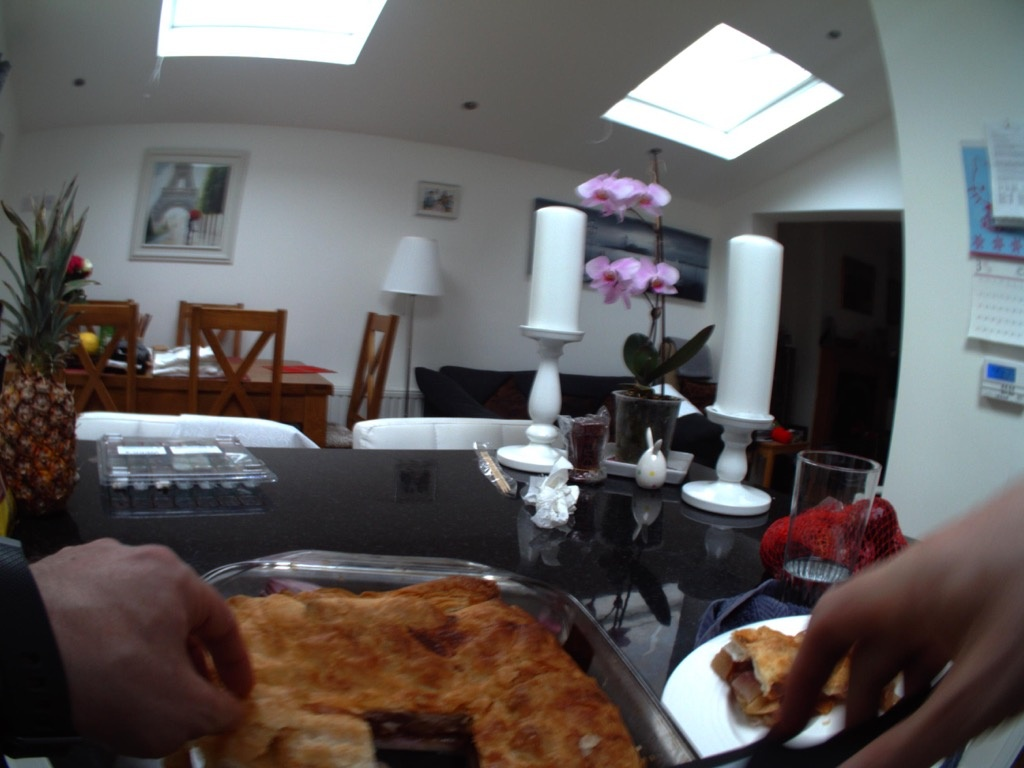
\includegraphics[width=\textwidth]{Sections/7Results/images/run3top2.jpg}\hfill
          \caption{Top 2}
        \end{subfigure}
          \begin{subfigure}{0.32\textwidth}
          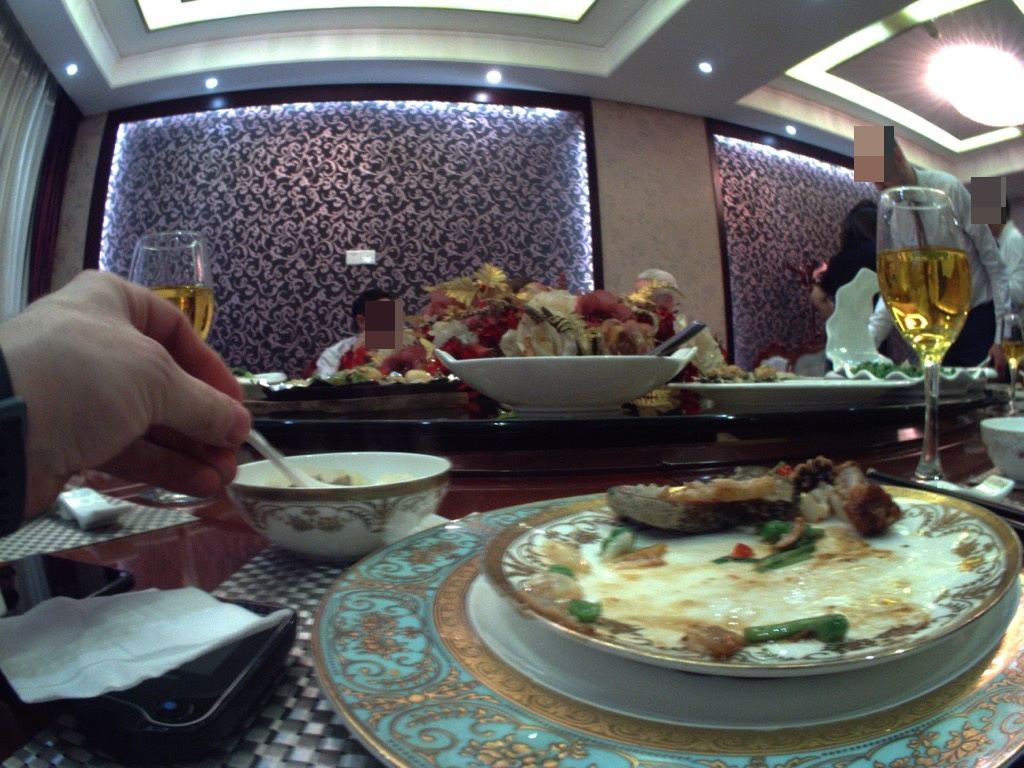
\includegraphics[width=\textwidth]{Sections/7Results/images/run2top3.jpg}\hfill
            \caption{Top 3}
        \end{subfigure} \par\medskip


      \begin{subfigure}{0.32\textwidth}
        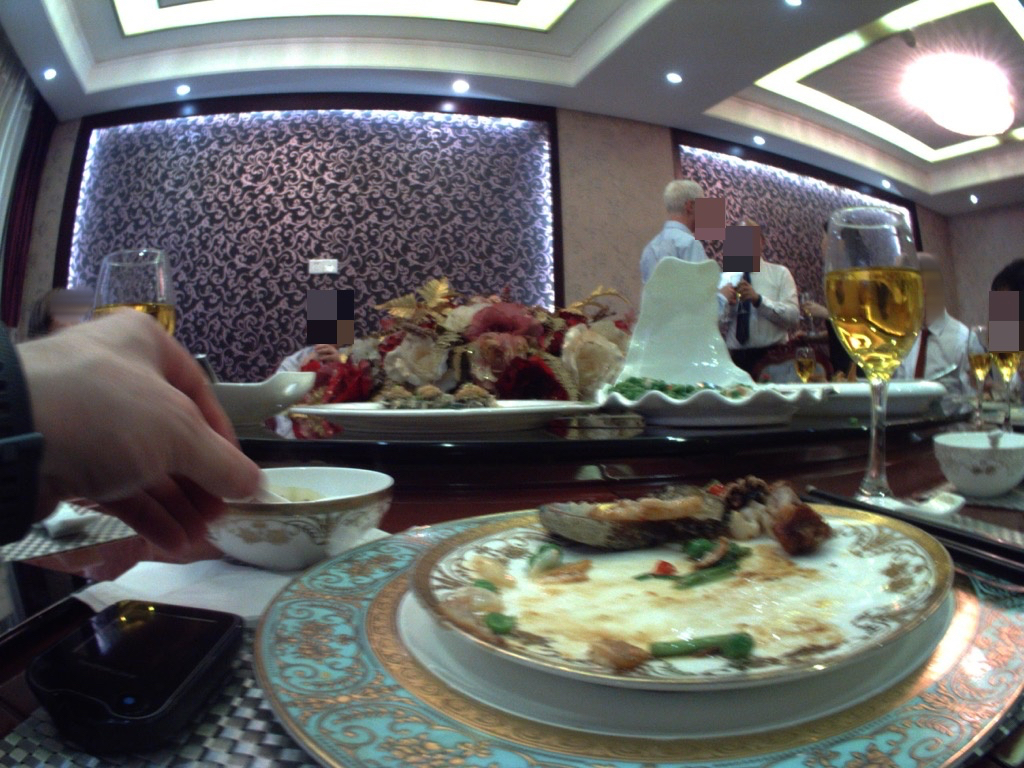
\includegraphics[width=\textwidth]{Sections/7Results/images/run2top4.jpg}\hfill
        \caption{Top 4}
      \end{subfigure}
      \begin{subfigure}{0.32\textwidth}
        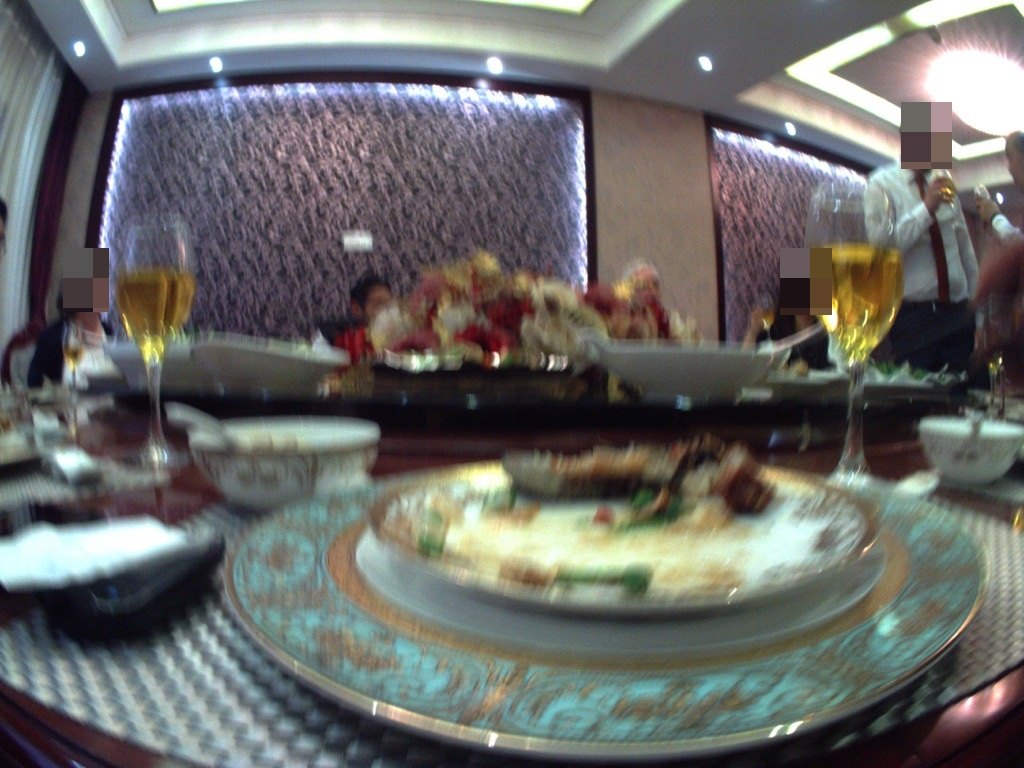
\includegraphics[width=\textwidth]{Sections/7Results/images/run2top5.jpg}\hfill
        \caption{Top 5}
      \end{subfigure}
      \begin{subfigure}{0.32\textwidth}
        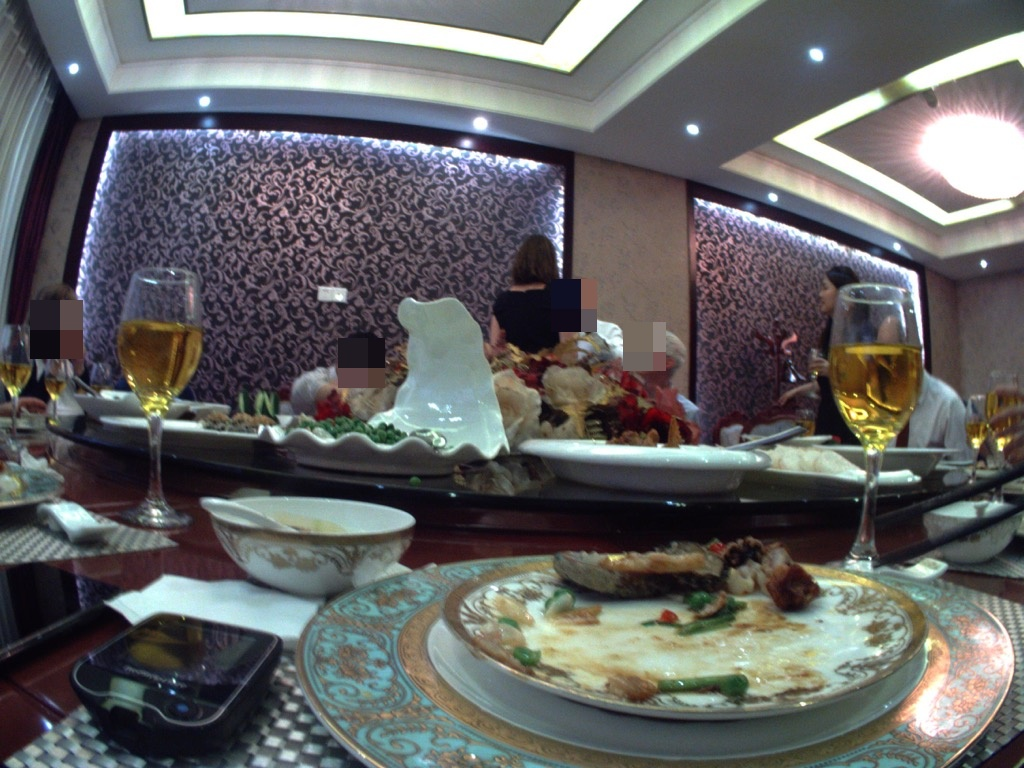
\includegraphics[width=\textwidth]{Sections/7Results/images/run2top6.jpg}\hfill
        \caption{Top 6}
      \end{subfigure}\par\medskip
      \begin{subfigure}{0.32\textwidth}
        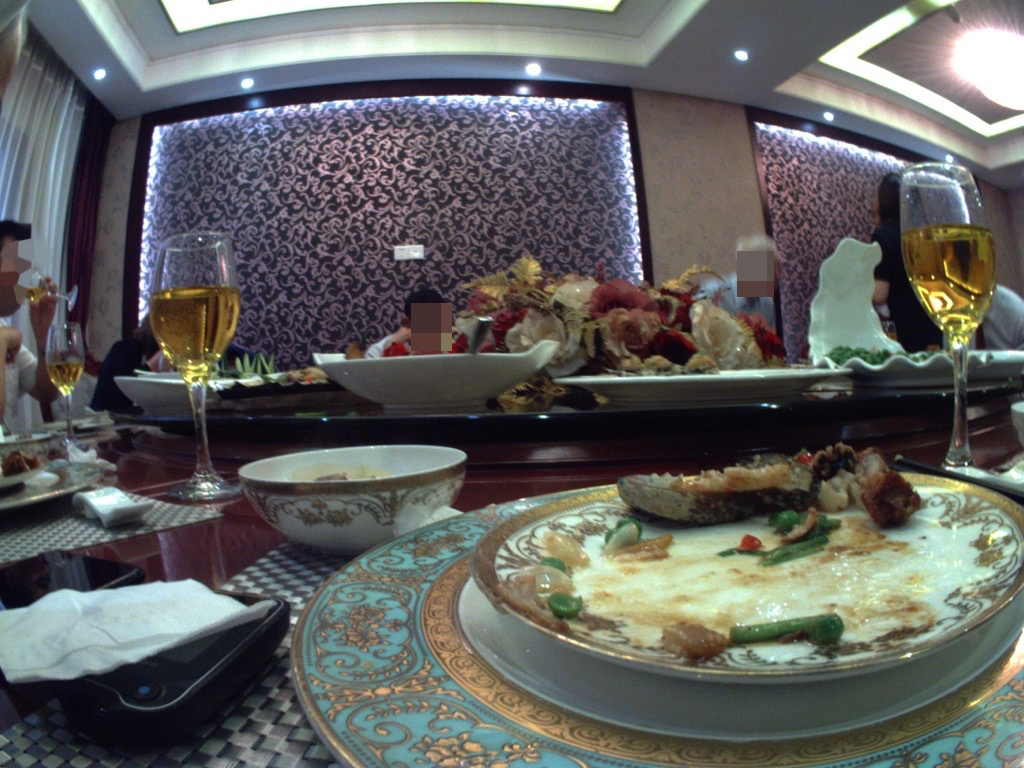
\includegraphics[width=\textwidth]{Sections/7Results/images/run2top7.jpg} 
        \caption{Top 7}
      \end{subfigure}
      \begin{subfigure}{0.32\textwidth}
        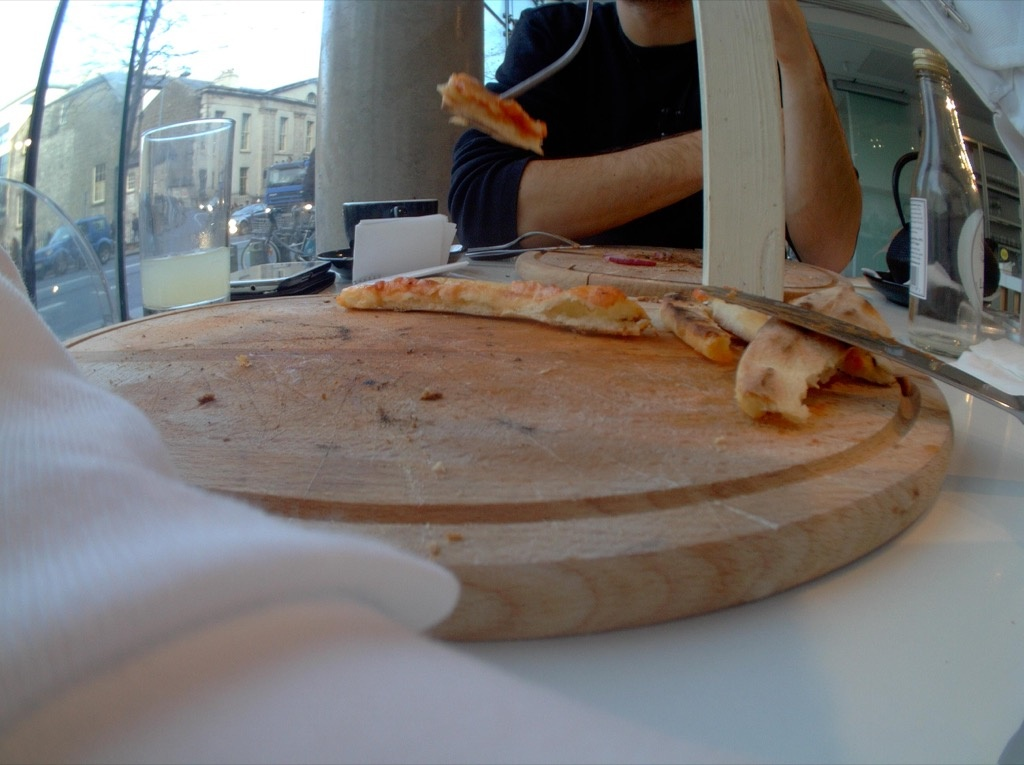
\includegraphics[width=\textwidth]{Sections/7Results/images/run2top8.jpg}\hfill
        \caption{Top 8}
      \end{subfigure}
      \begin{subfigure}{0.32\textwidth}
        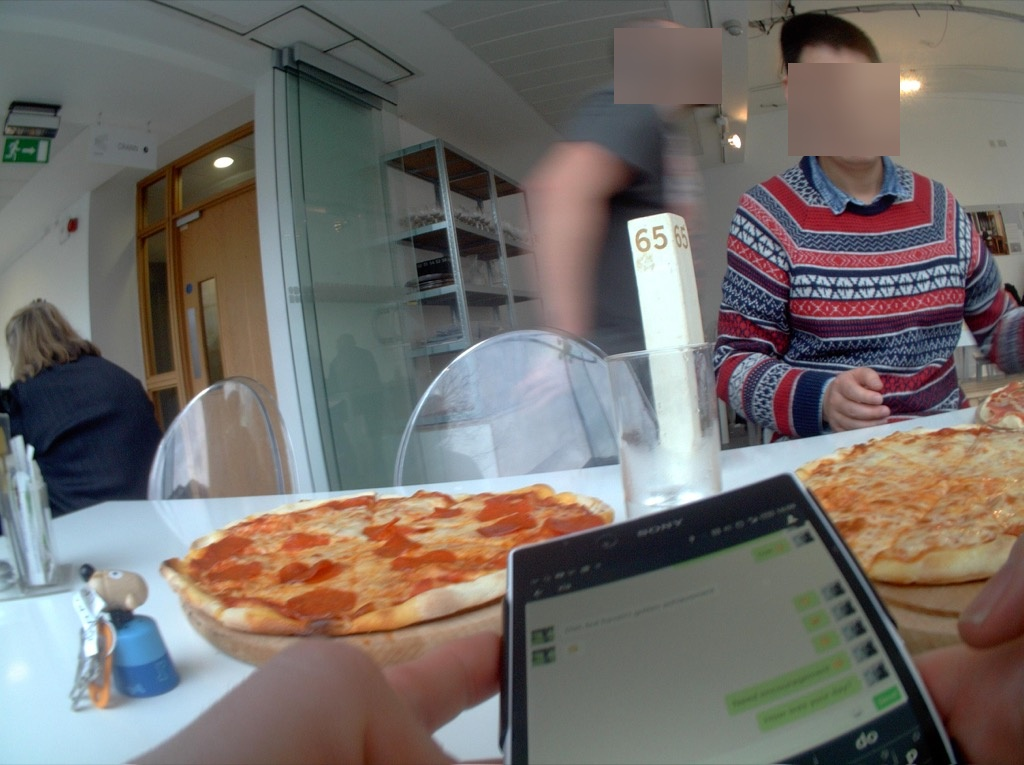
\includegraphics[width=\textwidth]{Sections/7Results/images/run2top9.jpg}\hfill
        \caption{Top 9}
      \end{subfigure} \par\medskip
      \begin{subfigure}{0.32\textwidth}
        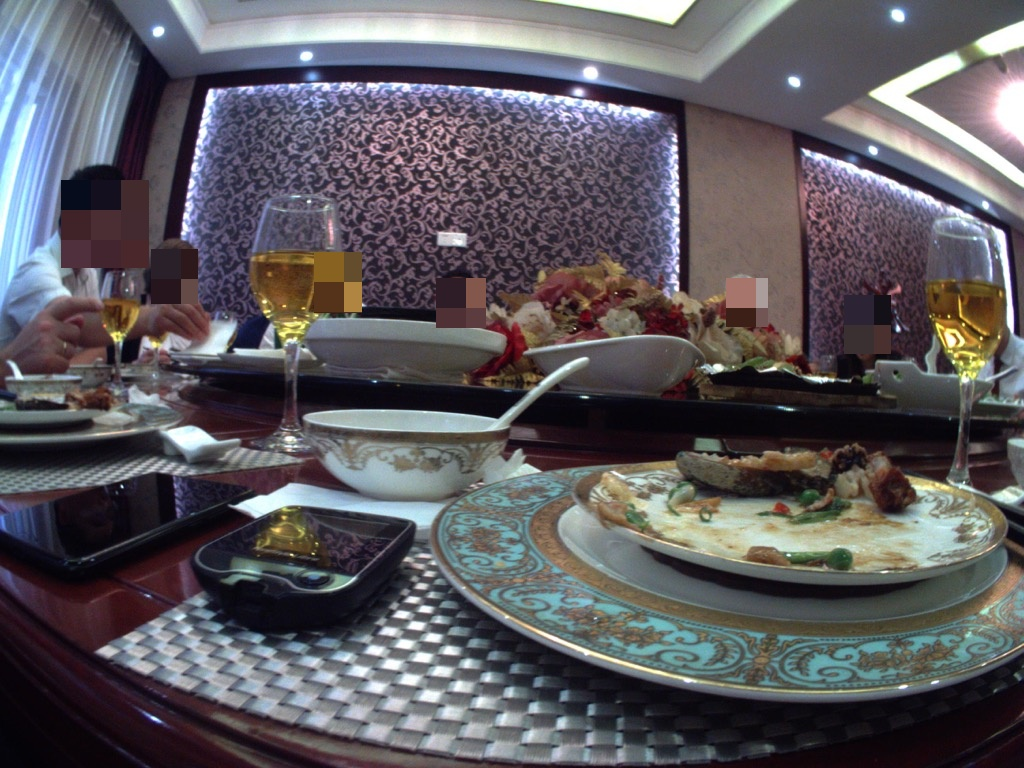
\includegraphics[width=\textwidth]{Sections/7Results/images/run2top10.jpg}\hfill
        \caption{Top 10}
      \end{subfigure}
    \caption{Top 3 retrieved pictures for topic 9 on run 2}
    \label{fig:run2}
  \end{figure}





  \newpage

 
\newpage

\section{Achieved Overall Performance Results}
\label{sec:perfomance_results}

Tables \ref{table:2019} and \ref{table:2020} provide an overview of the performance results achieved in different runs for different systems that were obtained in the year 2019 and 2020 for the ImageCLEFlifelog LMRT subtask. 
\newcolumntype{P}[1]{>{\centering\arraybackslash}p{#1}}
\begin{table}[H]
    
    \centering
\begin{tabular}{ |P{4cm}|P{2.5cm}|P{2cm}|P{3cm}|  }
    \hline
    \multicolumn{4}{|c|}{\textbf{2019 Results}} \\
    \hline
    Team & System Type & Run Name & F1-measure@10 \\
    \hline
    UA.PT Bioinformatics  & automatic  & Run 1   &  0.016 \\
    UA.PT Bioinformatics  & automatic  & Run 2   &  0.026 \\
    UA.PT Bioinformatics  & automatic  & Run 3   &  0.027 \\
    UA.PT Bioinformatics  & automatic  & Run 4   &  0.027 \\
    UA.PT Bioinformatics  & automatic  & Run 5   &  0.036 \\
    UA.PT Bioinformatics  & automatic  & Run 6   &  \textbf{0.057} \\
    \hline
    \multicolumn{4}{|c|}{\textbf{Best Results Achieved by a Team}} \\
    \hline
    HCMUS  & interactive  & Run 2   &  \textbf{0.61} \\
    \hline        
    \end{tabular}
    \caption[Results obtained in 2019]{Results obtained in 2019 from UA.PT Bioinformatics \cite{Ribeiro2019} and the best team \cite{Le2019}. }
    \label{table:2019}
\end{table}
\begin{table}[H]
    \centering
\begin{tabular}{ |P{4cm}|P{2.5cm}|P{2cm}|P{3cm}|  }   
    \hline
    \multicolumn{4}{|c|}{\textbf{2020 Results}} \\
    \hline
    Team & System Type & Run Name & F1-measure@10 \\
    \hline
    UA.PT Bioinformatics  & automatic  & Run 1   &  0.031 \\
    UA.PT Bioinformatics  & automatic  & Run 2   &  0.031 \\
    UA.PT Bioinformatics  & interactive  & Run 3  &  \textbf{0.517} \\
    \hline
    \multicolumn{4}{|c|}{\textbf{Best Results Achieved by a Team}} \\
    \hline
    HCMUS  & interactive  & Run 10   &  \textbf{0.81}\\
    \hline       
    \end{tabular}
    \caption[Results obtained in 2020]{Results obtained in 2020 from UA.PT Bioinformatics \cite{Ribeiro2020} and the best team \cite{Ninh2020}.}
    \label{table:2020}
\end{table}

\subsection{Overall Performance Analysis}
\label{sec:overall_perfomance}

Comparing the Table \ref{table:2019} that shows the results of the year 2019 and Table \ref{table:2020} that shows the results of this year challenge, it is clear that there was no overall improvement on an automatic system performance. Furthermore, it is also possible to clearly see the difference in performance between interactive systems and fully automatic systems. Having user interaction and visualizations yields much better results than a fully automatic system \cite{Ribeiro2020}.


The tables shown make a strong argument that for the ImageCLEF LMRT sub-task an interactive approach is a much better suited method, the user visualization and interaction with the application allows for much more accurate results since the user can manually choose the picture that he thinks is correct for the corresponding moment.

Another important aspect to notice is that the results of the automatic approach this year achieved the same exact F1-measure@10 score, this is highly due to the fact that even when using different state-of-the-art object detection algorithms, different weights for each category and even using negative categories on one run and not on the other, much of the data used for both runs was provided by the organizers which is a highly faulty and inaccurate.



The interactive system is built around a web application where the user has interaction with 3 different stages of the application. These stages are upload, retrieval and visualization. 

In the upload, the user uploads the dataset to be processed. During the retrieval stage, the user inputs the words extracted from the query topic into several categories and a comparison is done with the inputs and the app database information. This comparison is done in order to compute a confidence for each image for the assigned topic. Finally, in the visualization stage the user visualizes the images retrieved in forms of image gallery or data tables and manually selects the relevant clusters for the query topic. In order to improve the results, the user can exclude several irrelevant images from the selected clusters. To improve the cluster recall of the run, the user can change the confidence of a relevant image of each selected timestamp clusters \cite{Ribeiro2020}.

This last visualization step is the critical difference between both systems. In the interactive system the the user can exclude images that he thinks that do not belong to the moment described in the query topic. This makes the automatic system incapable of competing with the results of the interactive system.

Figure \ref{fig:app_view} shows a screenshot of the application retrieval view and Figure \ref{fig:app_diagram} illustrates the different stages presented in the interactive system 

\begin{figure}[H]
  \centering
  \captionsetup{justification=centering}

  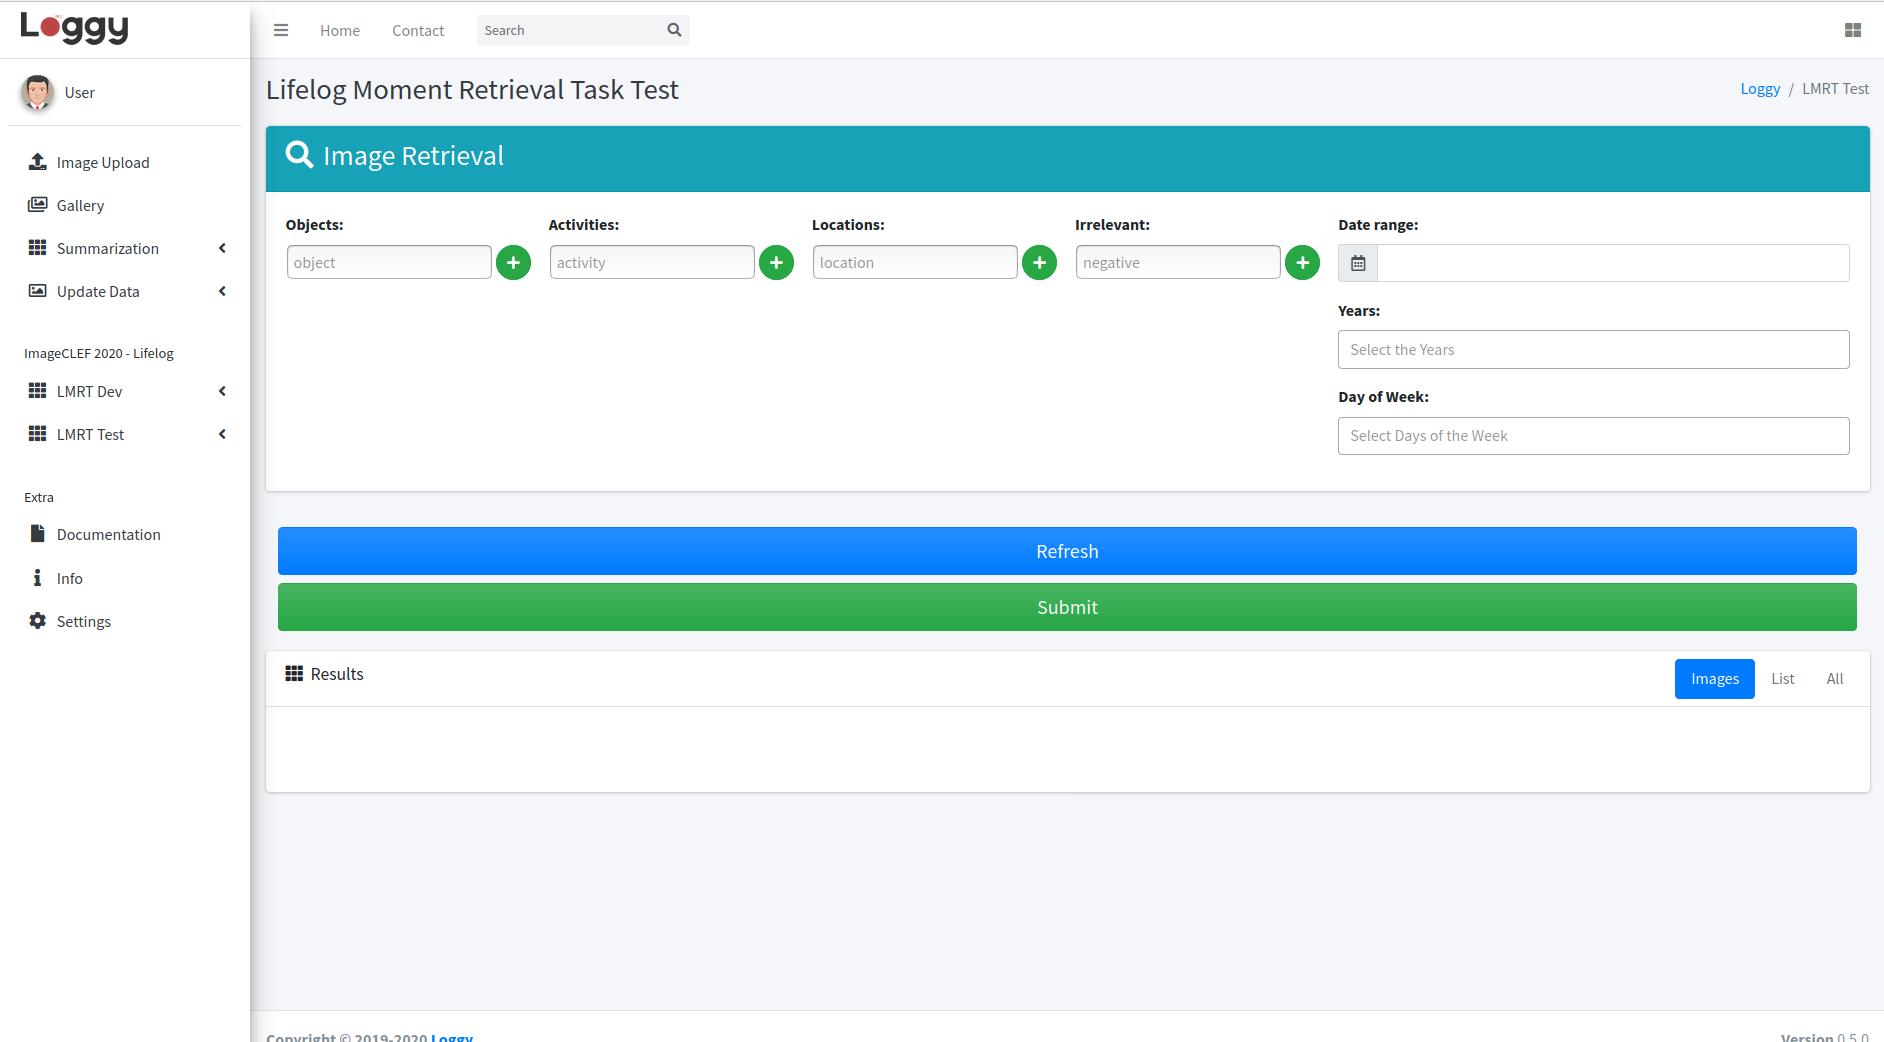
\includegraphics[width=\textwidth]{Sections/7Results/images/retrievalview.png} 
  \caption[Web application retrievable view] {Web application retrieval view \cite{Ribeiro2020}.}
  \label{fig:app_view}
\end{figure}

\begin{figure}[H]
  \centering
  \captionsetup{justification=centering}

  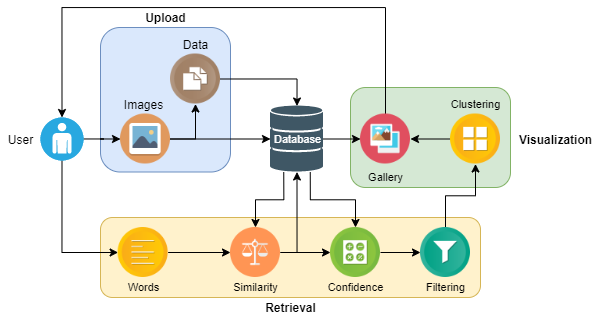
\includegraphics[width=0.75\textwidth]{Sections/7Results/images/Appdiagram.png} 
  \caption[General representation of the  developed  web  application.]{General representation of the  developed  web  application.  The  user  interacts with the three stages of the application: Upload, Retrieval and Visualization \cite{Ribeiro2020}.}
  \label{fig:app_diagram}
\end{figure}


